\documentclass[UTF8,11pt,a4paper,fontset=fandol]{ctexart}

\usepackage[a4paper,margin=2.1cm,headheight=15pt]{geometry}
\usepackage[table]{xcolor}
\usepackage{amsmath,amssymb}
\usepackage{booktabs,longtable,tabularx,array,multirow}
\usepackage{graphicx}
\usepackage{float}
\usepackage{tikz}
\usetikzlibrary{arrows.meta,positioning,shapes.geometric,fit,calc,backgrounds}
\usepackage{pgfplots}
\pgfplotsset{compat=1.18}
\usepackage{listings}
\usepackage{hyperref}
\usepackage{fancyhdr}
\usepackage{enumitem}

\definecolor{NvidiaGreen}{HTML}{76B900}
\definecolor{DeepBlue}{HTML}{245A8D}
\definecolor{LightBlue}{HTML}{DCEEFF}
\definecolor{LightGreen}{HTML}{E7F4CE}
\definecolor{WarmOrange}{HTML}{E58E26}
\definecolor{SoftRed}{HTML}{C94C4C}
\definecolor{CodeBg}{HTML}{F5F7FA}
\definecolor{GridGray}{HTML}{D8DEE9}

\hypersetup{
  colorlinks=true,
  linkcolor=DeepBlue,
  urlcolor=DeepBlue,
  citecolor=NvidiaGreen,
  pdftitle={GEMM Auto-Tuning 与 Nsight Compute Roofline 分析},
  pdfauthor={gemm-opt project}
}

\pagestyle{fancy}
\fancyhf{}
\lhead{GEMM Auto-Tuning 与 NCU Roofline 分析}
\rhead{RTX 4060 Laptop GPU}
\cfoot{\thepage}

\setlength{\parindent}{2em}
\setlength{\parskip}{0.35em}
\setlength{\emergencystretch}{2em}
\setlist{itemsep=0.2em,topsep=0.3em}
\renewcommand{\arraystretch}{1.18}
\newcommand{\code}[1]{\nolinkurl{#1}}

\lstdefinestyle{cuda}{
  language=C++,
  basicstyle=\ttfamily\small,
  keywordstyle=\color{DeepBlue}\bfseries,
  commentstyle=\color{NvidiaGreen!70!black},
  stringstyle=\color{WarmOrange!80!black},
  backgroundcolor=\color{CodeBg},
  frame=single,
  rulecolor=\color{GridGray},
  numbers=left,
  numberstyle=\tiny\color{gray},
  numbersep=8pt,
  breaklines=true,
  columns=fullflexible,
  showstringspaces=false,
  tabsize=4
}

\tikzset{
  process/.style={
    rectangle,rounded corners=2mm,draw=DeepBlue,very thick,
    fill=LightBlue,minimum width=2.7cm,minimum height=1.05cm,
    align=center,font=\small
  },
  analysis/.style={
    rectangle,rounded corners=2mm,draw=NvidiaGreen!70!black,very thick,
    fill=LightGreen,minimum width=2.7cm,minimum height=1.05cm,
    align=center,font=\small
  },
  arrow/.style={-{Latex[length=2.7mm]},very thick,draw=gray!75!black},
  memory/.style={rectangle,rounded corners,draw=DeepBlue,thick,fill=LightBlue,
    minimum width=2.45cm,minimum height=0.9cm,align=center},
  compute/.style={rectangle,rounded corners,draw=NvidiaGreen!70!black,thick,
    fill=LightGreen,minimum width=2.45cm,minimum height=0.9cm,align=center}
}

\title{\bfseries 基于 Nsight Compute 与 Roofline 的\\
参数化 GEMM Auto-Tuning 性能分析}
\author{gemm-opt CUDA 优化项目}
\date{2026 年 9 月 4 日}

\begin{document}

\begin{titlepage}
  \centering
  \vspace*{2.2cm}
  {\Huge\bfseries 基于 Nsight Compute 与 Roofline 的\par}
  \vspace{0.5cm}
  {\Huge\bfseries 参数化 GEMM Auto-Tuning 性能分析\par}
  \vspace{1.5cm}
  {\Large NVIDIA GeForce RTX 4060 Laptop GPU\par}
  \vspace{0.4cm}
  {\large CUDA 13 · cuBLAS 13 · Nsight Compute 2026.2.1\par}

  \vfill
  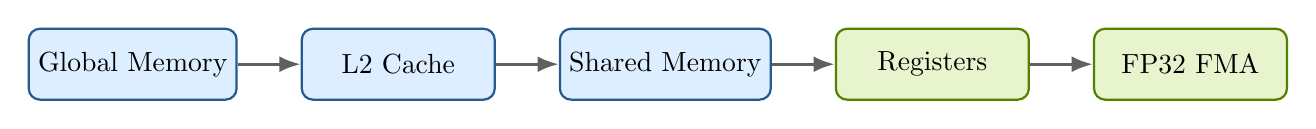
\begin{tikzpicture}[scale=1.0]
    \node[memory] (dram) {Global Memory};
    \node[memory,right=8mm of dram] (l2) {L2 Cache};
    \node[memory,right=8mm of l2] (smem) {Shared Memory};
    \node[compute,right=8mm of smem] (reg) {Registers};
    \node[compute,right=8mm of reg] (fma) {FP32 FMA};
    \draw[arrow] (dram)--(l2);
    \draw[arrow] (l2)--(smem);
    \draw[arrow] (smem)--(reg);
    \draw[arrow] (reg)--(fma);
  \end{tikzpicture}

  \vfill
  {\large gemm-opt CUDA 优化项目\par}
  \vspace{0.3cm}
  {\large 2026 年 9 月 4 日\par}
\end{titlepage}

\begin{abstract}
本文完整记录一个教学型 FP32 GEMM 从参数化实现、自动搜索、cuBLAS 对照，到 Nsight Compute（NCU）硬件计数器分析的全过程。Auto-Tuner 搜索 11 组 \code{BM/BN/BK/TM/TN} 参数，并在 $256^3$ 至 $4096^3$ 五种规模上与严格 FP32 cuBLAS、TF32 cuBLAS 比较。进一步选取低 Occupancy 的大 tile 最优配置和高 Occupancy 的小 tile 配置进行 NCU 对照，分析 DRAM/L2 流量、寄存器压力、Occupancy、Scheduler 状态及九类 Warp Stall。结果表明，大 tile 虽然仅有 16.67\% Occupancy，但依靠更高的片上数据复用将 L2 流量减半，并比 79.73\% Occupancy 的小 tile 更快。Roofline 分析显示该问题远离 DRAM 带宽边界，主要瓶颈位于片上 shared-memory/MIO 管线与指令依赖，而不是显存带宽。

\textbf{关键词：} CUDA；GEMM；Auto-Tuning；Nsight Compute；Roofline；Occupancy；Warp Stall；cuBLAS
\end{abstract}

\tableofcontents
\newpage

\section{目标与完整工作流}

本实验的目标不是只给出一个最快参数，而是建立一条可重复的性能工程流程：首先用统一模板表达搜索空间；其次把正确性与性能计时分离；然后用 cuBLAS 建立参考线；最后只对最有代表性的 kernel 采集昂贵的硬件计数器。

\begin{figure}[H]
\centering
\resizebox{\textwidth}{!}{%
\begin{tikzpicture}[node distance=9mm and 10mm]
  \node[process] (source) {参数化 CUDA kernel\\\code{BM/BN/BK/TM/TN}};
  \node[process,right=of source] (compile) {编译候选配置\\读取 Reg/SMEM};
  \node[process,right=of compile] (bench) {预热 + CUDA Event\\多次重复计时};
  \node[analysis,right=of bench] (verify) {cuBLAS FP32 参考\\逐元素正确性检查};
  \node[analysis,below=12mm of verify] (select) {按矩阵规模\\选择最优配置};
  \node[analysis,left=of select] (ncu) {NCU 过滤单 kernel\\17-pass replay};
  \node[analysis,left=of ncu] (roof) {Roofline / 带宽\\Occupancy / Stall};
  \node[analysis,left=of roof] (report) {CSV + NCU report\\LaTeX/PDF 报告};

  \draw[arrow] (source)--(compile);
  \draw[arrow] (compile)--(bench);
  \draw[arrow] (bench)--(verify);
  \draw[arrow] (verify)--(select);
  \draw[arrow] (select)--(ncu);
  \draw[arrow] (ncu)--(roof);
  \draw[arrow] (roof)--(report);
\end{tikzpicture}}
\caption{从参数化实现到性能结论的完整流程}
\label{fig:workflow}
\end{figure}

整个过程遵循两条原则：

\begin{enumerate}
  \item \textbf{普通运行负责计时。} NCU 为收集多组计数器会 replay kernel，本次每个目标执行 17 个 pass，因此不能把 profiler 下的 wall time 当作最终 GFLOPS。
  \item \textbf{NCU 负责解释原因。} 使用同规模、同指标集合对照两个参数配置，通过寄存器、Occupancy、数据流量和 Stall 解释性能差异。
\end{enumerate}

\section{实验环境与工具准备}

\subsection{硬件与软件}

\begin{table}[H]
\centering
\caption{实验环境}
\begin{tabular}{ll}
\toprule
项目 & 实测值 \\
\midrule
GPU & NVIDIA GeForce RTX 4060 Laptop GPU \\
Compute Capability & 8.9（Ada） \\
SM 数量 & 24 \\
显存容量 / 总线 & 8188 MiB / 128 bit \\
NVIDIA Driver & 595.84 \\
CUDA 编译器 & CUDA 13.0.88 \\
cuBLAS & \code{libcublas.so.13} \\
Nsight Compute & 2026.2.1 \\
Nsight Systems & 2026.4.1 \\
NCU 采样时钟 & SM 1.89 GHz，DRAM 7.99 GHz \\
GPU 功耗限制 & 当前 50 W，requested 55 W \\
\bottomrule
\end{tabular}
\end{table}

\subsection{工具安装问题与解决过程}

系统原有 NCU 2021.3.1 可以连接进程，但在 CUDA API 调用处返回 ``API call is not supported in the installed CUDA driver''，无法对 CUDA 13 和 Ada GPU 生成可信报告。因此改用支持 Ada 的 NCU 2026.2.1\cite{ncu-download}。

根分区空间不足，而 \code{/media/drink_ice/Data} 最初因为 Windows 快速启动/休眠残留处于 NTFS unsafe state，被 Linux 保护性地只读挂载。关闭 Windows 休眠并完整关机后，分区恢复为读写模式。随后：

\begin{itemize}
  \item NCU 安装到 \code{/media/drink_ice/Data/cuda-tools/nsight-compute-2026.2.1}；
  \item NCU 原始报告写入 \code{/media/drink_ice/Data/gemm-opt-profiles/ncu}；
  \item Nsight Systems 迁移到 Data 分区，原目录改为软链接；
  \item 根分区释放约 607 MB，项目中的 \code{.tools} 只保留软链接。
\end{itemize}

pip 版 CUDA 13 还缺少 \code{nv/target}，因此将 NVIDIA CCCL 头文件安装到 Data 分区，并通过 Makefile 的额外 include 路径编译；cuBLAS Python 包只有版本化 DSO，链接时使用 \code{-l:libcublas.so.13}，不修改系统库目录。

\section{参数化 GEMM 的实现}

\subsection{矩阵分块与 K 方向}

GEMM 定义为
\begin{equation}
  C_{M\times N}=A_{M\times K}B_{K\times N},\qquad
  C_{ij}=\sum_{k=0}^{K-1}A_{ik}B_{kj}.
\end{equation}

所谓 K 方向，就是求和下标 $k$ 延伸的方向。每次不必把完整的 K 都放入 shared memory，而是取长度为 \code{BK} 的切片；所有线程完成这一片的乘加后，再进入下一片。

\begin{figure}[H]
\centering
\begin{tikzpicture}[x=0.075cm,y=0.075cm,font=\small]
  % A
  \draw[thick] (0,0) rectangle (64,45);
  \fill[LightBlue] (0,22) rectangle (64,34);
  \draw[DeepBlue,very thick] (0,22) rectangle (64,34);
  \node at (32,49) {$A\;(M\times K)$};
  \node[rotate=90] at (-5,22.5) {$M$};
  \node at (32,-5) {$K$};
  \node at (32,28) {$BM\times BK$};

  % B
  \draw[thick] (78,0) rectangle (123,45);
  \fill[LightGreen] (88,0) rectangle (105,45);
  \draw[NvidiaGreen!70!black,very thick] (88,0) rectangle (105,45);
  \node at (100.5,49) {$B\;(K\times N)$};
  \node[rotate=90] at (73,22.5) {$K$};
  \node at (100.5,-5) {$N$};
  \node[rotate=90] at (96.5,22.5) {$BK\times BN$};

  % arrow
  \draw[arrow] (64,28) -- node[above] {沿 K 对齐并乘加} (78,28);

  % C
  \draw[thick] (139,0) rectangle (184,45);
  \fill[WarmOrange!25] (149,22) rectangle (166,34);
  \draw[WarmOrange,very thick] (149,22) rectangle (166,34);
  \node at (161.5,49) {$C\;(M\times N)$};
  \node[rotate=90] at (134,22.5) {$M$};
  \node at (161.5,-5) {$N$};
  \node at (157.5,28) {$BM\times BN$};

  \draw[decorate,decoration={brace,amplitude=5pt},DeepBlue]
    (0,19)--(64,19) node[midway,below=6pt] {BK 切片沿 K 方向依次移动};
\end{tikzpicture}
\caption{一个 block 使用 $BM\times BK$ 的 A tile 和 $BK\times BN$ 的 B tile，累加一个 $BM\times BN$ 的 C tile}
\label{fig:tiling}
\end{figure}

\subsection{五个调优参数}

\begin{table}[H]
\centering
\caption{模板参数的作用}
\begin{tabularx}{\textwidth}{cX}
\toprule
参数 & 含义及主要影响 \\
\midrule
\code{BM} & 一个 thread block 输出 C tile 的行数；增大它会增加 A 的复用和 shared-memory 用量。 \\
\code{BN} & 一个 thread block 输出 C tile 的列数；增大它会增加 B 的复用和 shared-memory 用量。 \\
\code{BK} & 一次 global-to-shared 加载覆盖的 K 长度；影响同步次数、循环开销和 shared-memory 容量。 \\
\code{TM} & 每线程输出的行数；与 \code{TN} 一起决定累加器数量和寄存器压力。 \\
\code{TN} & 每线程输出的列数；增大它可提高 ILP，但也可能显著降低 Occupancy。 \\
\bottomrule
\end{tabularx}
\end{table}

核心模板定义如下：

\begin{lstlisting}[style=cuda,caption={参数化 GEMM kernel 的结构}]
template <int BM, int BN, int BK, int TM, int TN>
__global__ void gemmTunable(const float* A, const float* B,
                            float* C, int M, int N, int K) {
    __shared__ float tileA[BM][BK + 1];
    __shared__ float tileB[BK][BN];
    float accum[TM][TN] = {};

    for (int tileK = 0; tileK < K; tileK += BK) {
        // cooperative float4 global -> shared loads
        loadATileFloat4(...);
        loadBTileFloat4(...);
        __syncthreads();

        #pragma unroll
        for (int k = 0; k < BK; ++k) {
            float regA[TM], regB[TN];
            loadFromShared(regA, regB, tileA, tileB, k);
            outerProductFma(accum, regA, regB);
        }
        __syncthreads();
    }
    storeResultWithBoundsCheck(C, accum, M, N);
}
\end{lstlisting}

实际源码没有调用上面三个示意函数，而是将它们完全展开，以便编译器进行 unroll 和寄存器分配。

\subsection{数据层级和复用}

\begin{figure}[H]
\centering
\resizebox{\textwidth}{!}{%
\begin{tikzpicture}[node distance=11mm]
  \node[memory] (global) {Global Memory\\A、B、C};
  \node[memory,right=of global] (l2) {L2 Cache\\跨 block 缓存};
  \node[memory,right=of l2] (shared) {Shared Memory\\$BM\times BK$ / $BK\times BN$};
  \node[compute,right=of shared] (regs) {Registers\\$TM+TN+TM\times TN$};
  \node[compute,right=of regs] (fma) {FP32 FMA\\Outer Product};

  \draw[arrow] (global)--node[above,font=\scriptsize]{\code{float4}}(l2);
  \draw[arrow] (l2)--node[above,font=\scriptsize]{合作加载}(shared);
  \draw[arrow] (shared)--node[above,font=\scriptsize]{广播/复用}(regs);
  \draw[arrow] (regs)--node[above,font=\scriptsize]{寄存器操作数}(fma);
  \draw[-{Latex},thick,WarmOrange,bend right=35] (fma.south) to node[below,font=\scriptsize]{累加 $TM\times TN$ 次}(regs.south);
\end{tikzpicture}}
\caption{参数化 kernel 的存储层级。优化目标是让每个更昂贵的上层字节服务更多 FMA。}
\label{fig:memory-hierarchy}
\end{figure}

具体实现还包括：

\begin{itemize}
  \item 使用 16 Byte 对齐的 \code{float4} 读取 A、B；边界不足四个元素时回退为标量补零；
  \item A tile 定义为 \code{tileA[BM][BK+1]}，用一列 padding 改变 shared-memory 行跨度；
  \item 每个线程维护 $TM\times TN$ 个累加器，并在一个 $k$ 步内执行 outer product；
  \item 输出阶段执行边界判断，因此框架可继续扩展到非 tile 整数倍规模。
\end{itemize}

\section{Auto-Tuning 框架与正确性验证}

\subsection{候选空间}

所有候选都使用 256 threads/block，改变 block tile、K tile 和 thread tile。编译后通过 CUDA Runtime 查询真实寄存器和静态 shared-memory 用量，再调用 Occupancy API 计算理论值。

\begin{longtable}{cccccc}
\caption{候选参数、资源占用与 2048\textsuperscript{3} 性能}\label{tab:candidates}\\
\toprule
$BM\times BN\times BK$ & $TM\times TN$ & Reg/thread & Shared/block & 理论 Occ. & GFLOPS \\
\midrule
\endfirsthead
\toprule
$BM\times BN\times BK$ & $TM\times TN$ & Reg/thread & Shared/block & 理论 Occ. & GFLOPS \\
\midrule
\endhead
32$\times$32$\times$8   & 2$\times$2 & 38  & 2.13 KiB  & 100.0\% & 1572.7 \\
64$\times$64$\times$8   & 4$\times$4 & 48  & 4.25 KiB  & 83.3\%  & 3182.9 \\
64$\times$64$\times$16  & 4$\times$4 & 48  & 8.25 KiB  & 83.3\%  & 3107.3 \\
64$\times$64$\times$32  & 4$\times$4 & 48  & 16.25 KiB & 83.3\%  & 3121.3 \\
64$\times$128$\times$8  & 4$\times$8 & 90  & 6.25 KiB  & 33.3\%  & 3386.6 \\
64$\times$128$\times$16 & 4$\times$8 & 80  & 12.25 KiB & 50.0\%  & 3882.8 \\
128$\times$64$\times$8  & 8$\times$4 & 64  & 6.50 KiB  & 66.7\%  & 3654.7 \\
128$\times$64$\times$16 & 8$\times$4 & 63  & 12.50 KiB & 66.7\%  & 3944.3 \\
128$\times$128$\times$8 & 8$\times$8 & 168 & 8.50 KiB  & 16.7\%  & 3964.0 \\
128$\times$128$\times$16& 8$\times$8 & 153 & 16.50 KiB & 16.7\%  & 4219.4 \\
\rowcolor{LightGreen}
128$\times$128$\times$32& 8$\times$8 & 158 & 32.50 KiB & 16.7\%  & \textbf{4343.7} \\
\bottomrule
\end{longtable}

\subsection{计时与正确性}

每个配置先预热 5 次，再用 CUDA Event 对多次连续调用计时。不同规模的重复次数分别为 100、100、50、20、10。输入初始化、Host--Device 拷贝以及逐元素误差检查都在计时区间之外。

cuBLAS 使用列主序，因此 row-major 的 $C=AB$ 被解释为 $C^T=B^TA^T$，调用时交换 A、B 和 M、N。公平的 FP32 参考采用 \code{CUBLAS_COMPUTE_32F_PEDANTIC}；另测 \code{CUBLAS_COMPUTE_32F_FAST_TF32}，展示允许 Tensor Core 后的性能。两种 compute type 的定义见 cuBLAS 文档\cite{cublas-doc}。

自定义配置的容差为
\begin{equation}
  \epsilon = 10^{-3} + 10^{-4}\max_i |C_i^{\text{cuBLAS FP32}}|.
\end{equation}
五个规模、11 个候选全部通过；自定义 kernel 的记录最大绝对误差为 0。TF32 在本组输入上的最大绝对误差为 $4\times10^{-6}$ 至 $1.2\times10^{-5}$，但这不表示 TF32 对一般输入与严格 FP32 等价。

\section{多规模性能与 cuBLAS 对比}

\begin{table}[H]
\centering
\caption{五种方阵规模的最优结果}
\resizebox{\textwidth}{!}{%
\begin{tabular}{rccrrrr}
\toprule
$M=N=K$ & 最优 $BM\times BN\times BK$ & $TM\times TN$ & 自定义 GFLOPS & cuBLAS FP32 & 达到 cuBLAS & cuBLAS TF32 \\
\midrule
256  & 64$\times$64$\times$32   & 4$\times$4 & 1216.8 & 2899.8 & 42.0\% & 4206.4 \\
512  & 128$\times$128$\times$32 & 8$\times$8 & 3435.6 & 5435.3 & 63.2\% & 8126.0 \\
1024 & 128$\times$128$\times$32 & 8$\times$8 & \textbf{4433.2} & 8629.5 & 51.4\% & 14029.6 \\
2048 & 128$\times$128$\times$32 & 8$\times$8 & 4343.7 & 7757.5 & 56.0\% & 9509.5 \\
4096 & 128$\times$128$\times$32 & 8$\times$8 & 3582.0 & 5678.1 & 63.1\% & 11577.7 \\
\bottomrule
\end{tabular}}
\end{table}

\begin{figure}[H]
\centering
\begin{tikzpicture}
\begin{axis}[
  width=0.94\textwidth,height=8.0cm,
  symbolic x coords={256,512,1024,2048,4096},
  xtick=data,
  xlabel={$M=N=K$},ylabel={性能（GFLOPS）},
  ymin=0,ymax=15500,
  grid=major,grid style={draw=GridGray},
  legend style={at={(0.5,1.02)},anchor=south,legend columns=3},
  line width=1.2pt,mark size=2.7pt
]
\addplot[color=DeepBlue,mark=*] coordinates {
  (256,1216.8) (512,3435.6) (1024,4433.2) (2048,4343.7) (4096,3582.0)};
\addlegendentry{自定义 FP32}
\addplot[color=NvidiaGreen!70!black,mark=square*] coordinates {
  (256,2899.8) (512,5435.3) (1024,8629.5) (2048,7757.5) (4096,5678.1)};
\addlegendentry{cuBLAS FP32}
\addplot[color=WarmOrange,mark=triangle*] coordinates {
  (256,4206.4) (512,8126.0) (1024,14029.6) (2048,9509.5) (4096,11577.7)};
\addlegendentry{cuBLAS TF32}
\end{axis}
\end{tikzpicture}
\caption{自定义最优配置与 cuBLAS 的多规模性能曲线}
\label{fig:performance}
\end{figure}

结果可分为三个阶段：

\begin{enumerate}
  \item $256^3$ 时，128$\times$128 tile 只有 4 个 block，无法填满 24 个 SM；64$\times$64 tile 以更多 block 获胜。
  \item 从 $512^3$ 开始，并行度已经足够，128$\times$128 tile 的数据复用成为主导。
  \item cuBLAS 会按规模选择不同的内部 kernel/算法，而本框架只搜索同一教学 kernel 的 tile 参数；达到严格 FP32 cuBLAS 的 51\%--63\% 是合理结果。若允许 TF32，优化方向应转为 Tensor Core pipeline。
\end{enumerate}

\section{Nsight Compute 采集方法}

Auto-Tuner 的 \code{--profile CONFIG --size N} 模式只启动一个指定配置。程序执行 5 次 warmup 和 1 次目标 launch；NCU 使用相同 skip/count 精确过滤第 6 次 kernel：

\begin{lstlisting}[style=cuda,language=bash,caption={NCU 采集命令的核心参数}]
ncu \
  --kernel-name-base function \
  --kernel-name regex:gemmTunable \
  --launch-skip 5 --launch-count 1 \
  --section SpeedOfLight \
  --section SpeedOfLight_RooflineChart \
  --section LaunchStats \
  --section Occupancy \
  --section MemoryWorkloadAnalysis \
  --section SchedulerStats \
  --section WarpStateStats \
  --metrics dram__bytes_read.sum,dram__bytes_write.sum,... \
  ./bin/autotune_gemm --profile CONFIG --size 2048
\end{lstlisting}

除 section 自带指标外，还显式采集 DRAM read/write、L2 bytes、duration，以及 barrier、long/short scoreboard、MIO/LG throttle、math-pipe throttle、wait、not-selected、no-instruction 九类 Warp Stall。

本组 section 需要 17 次 kernel replay。NCU 文档指出，多指标只能分批采集，replay 前后还涉及保存/恢复可访问显存，因此 profiler 开销会随 section 和 kernel 数增加\cite{ncu-cli,ncu-overhead}。所以图~\ref{fig:performance} 使用独立 CUDA Event 数据，NCU duration 只用于同一采样条件下的微架构对照。

\section{Roofline 与内存带宽分析}

\subsection{模型和 ridge point}

Roofline 模型把性能上界写为\cite{ncu-roofline}：
\begin{equation}
  P \leq \min\left(P_{\mathrm{peak}},\; BW\times AI\right),
  \qquad AI=\frac{\mathrm{FLOP}}{\mathrm{Byte}}.
\end{equation}

以 NCU 的采样时钟估计：
\begin{align}
P_{\mathrm{FP32}} &\approx 24\times128\times2\times1.89
                     =11.61\ \mathrm{TFLOPS},\\
BW_{\mathrm{DRAM}} &\approx 2\times7.99\ \mathrm{GHz}
                     \times128\ \mathrm{bit}/8
                     =255.68\ \mathrm{GB/s},\\
AI_{\mathrm{ridge}} &\approx 11612/255.68
                     =45.4\ \mathrm{FLOP/Byte}.
\end{align}

Laptop GPU 会受功耗、温度和 boost 影响，上述值是采样时刻的 Roofline 估计，不是固定铭牌值。

\begin{figure}[H]
\centering
\begin{tikzpicture}
\begin{loglogaxis}[
  width=0.92\textwidth,height=8.3cm,
  xmin=1,xmax=1000,ymin=100,ymax=20000,
  xlabel={算术强度（FLOP/Byte）},ylabel={性能（GFLOPS）},
  grid=both,grid style={draw=GridGray},
  legend style={at={(0.02,0.98)},anchor=north west},
  log basis x=10,log basis y=10
]
\addplot[color=DeepBlue,very thick,domain=1:45.4,samples=50] {255.68*x};
\addlegendentry{DRAM bandwidth roof}
\addplot[color=NvidiaGreen!70!black,very thick,domain=45.4:1000,samples=2] {11612};
\addlegendentry{FP32 compute roof}
\addplot[only marks,mark=*,mark size=4pt,color=WarmOrange]
  coordinates {(390.7,3687)};
\addlegendentry{大 tile：128$\times$128$\times$32}
\addplot[only marks,mark=square*,mark size=4pt,color=SoftRed]
  coordinates {(388.2,2659)};
\addlegendentry{小 tile：64$\times$64$\times$16}
\addplot[dashed,gray,domain=45.4:45.4] coordinates {(45.4,100) (45.4,11612)};
\node[anchor=south west,font=\small] at (axis cs:47,140) {ridge $\approx45.4$};
\end{loglogaxis}
\end{tikzpicture}
\caption{2048\textsuperscript{3} 两个参数配置相对于 DRAM Roofline 的位置}
\label{fig:roofline}
\end{figure}

\subsection{DRAM 与 L2 流量}

一次 $2048^3$ GEMM 执行 $2\times2048^3=17.180$ GFLOP。两组 NCU 数据如下：

\begin{table}[H]
\centering
\caption{2048\textsuperscript{3} 的内存与 Roofline 指标}
\begin{tabular}{lrr}
\toprule
指标 & 大 tile 最优配置 & 小 tile 对照配置 \\
\midrule
NCU duration & 4.66 ms & 6.46 ms \\
NCU 推算性能 & 3.69 TFLOPS & 2.66 TFLOPS \\
NCU FP32 peak 百分比 & 32\% & 23\% \\
DRAM read & 33.69 MB & 33.73 MB \\
DRAM write & 10.28 MB & 10.53 MB \\
DRAM bandwidth & 9.44 GB/s & 6.86 GB/s \\
DRAM peak 利用率 & 3.69\% & 2.68\% \\
实测 DRAM AI & 390.7 FLOP/Byte & 388.2 FLOP/Byte \\
L2 traffic & 554.21 MB & 1.09 GB \\
L2 层 AI & 31.0 FLOP/Byte & 约 15.8 FLOP/Byte \\
L2 hit rate & 93.90\% & 96.88\% \\
\bottomrule
\end{tabular}
\end{table}

两个点的 DRAM AI 都远高于 45.4 FLOP/Byte 的 ridge point，且 DRAM 利用率不到 4\%，因此相对于显存带宽均属于 \textbf{compute-bound}。这里 NCU 的高 ``Memory Throughput'' 百分比主要来自片上 L1TEX/shared-memory/MIO 管线，不能误读成 DRAM 已经饱和。

每个 K tile 的理论片上算术强度为
\begin{equation}
AI_{\mathrm{tile}}=
\frac{2BM\cdot BN\cdot BK}
{4(BM\cdot BK+BK\cdot BN)}
=\frac{BM\cdot BN}{2(BM+BN)}.
\end{equation}

128$\times$128 tile 的理论值为 32 FLOP/Byte，与实测 L2 AI 31.0 接近；64$\times$64 tile 的理论值为 16，与实测约 15.8 接近。大 tile 的关键收益是把 L2 到片上层级的流量减少约一半。

\begin{figure}[H]
\centering
\begin{tikzpicture}
\begin{axis}[
  width=0.72\textwidth,height=7cm,
  ybar,bar width=22pt,
  symbolic x coords={大 tile,小 tile},xtick=data,
  ylabel={L2 traffic（MB）},ymin=0,ymax=1200,
  nodes near coords,
  nodes near coords align={vertical},
  grid=major,grid style={draw=GridGray}
]
\addplot[fill=DeepBlue!65,draw=DeepBlue] coordinates {(大 tile,554.21) (小 tile,1090)};
\end{axis}
\end{tikzpicture}
\caption{大 tile 通过更高复用将 L2 流量减半}
\label{fig:l2traffic}
\end{figure}

\section{寄存器压力与 Occupancy}

\begin{table}[H]
\centering
\caption{资源占用与 Occupancy 对照}
\begin{tabular}{lrr}
\toprule
指标 & 大 tile 最优配置 & 小 tile 对照配置 \\
\midrule
Registers/thread & 158 & 48 \\
Static shared/block & 33.28 KB & 8.45 KB \\
Register block limit/SM & 1 & 5 \\
Shared-memory block limit/SM & 1 & 6 \\
Theoretical active warps/SM & 8 & 40 \\
Theoretical Occupancy & 16.67\% & 83.33\% \\
Achieved Occupancy & 16.67\% & 79.73\% \\
Local/shared spilling & 0 & 0 \\
\bottomrule
\end{tabular}
\end{table}

大 tile 中每线程的 $8\times8=64$ 个 FP32 累加器是寄存器压力的主要来源；33.28 KB shared memory 也使每个 SM 只能驻留一个 block。它却依靠更高 ILP、更少 shared-memory 重复读取和更少同步获得更高性能，并且没有发生 spilling。

\begin{figure}[H]
\centering
\begin{tikzpicture}
\begin{axis}[
  width=0.75\textwidth,height=7cm,
  xmin=0,xmax=100,ymin=4,ymax=7,
  xlabel={Achieved Occupancy（\%）},ylabel={NCU duration（ms）},
  grid=major,grid style={draw=GridGray}
]
\addplot[only marks,mark=*,mark size=5pt,color=DeepBlue]
  coordinates {(16.67,4.66)};
\node[anchor=south west] at (axis cs:16.67,4.66) {大 tile：158 Reg/thread};
\addplot[only marks,mark=square*,mark size=5pt,color=SoftRed]
  coordinates {(79.73,6.46)};
\node[anchor=north east] at (axis cs:79.73,6.46) {小 tile：48 Reg/thread};
\end{axis}
\end{tikzpicture}
\caption{本实验中 Occupancy 更高的配置反而更慢}
\label{fig:occupancy-duration}
\end{figure}

这验证了 NVIDIA 的实践建议：Occupancy 反映延迟隐藏能力，但提高 Occupancy 不保证性能同比提高；低 Occupancy kernel 可能利用更多寄存器形成足够的 ILP\cite{cuda-best-practices}。因此不应直接用 \code{-maxrregcount} 压低寄存器，而应观察是否产生 spill，以及整体数据复用是否被破坏。

\section{Warp Scheduler 与 Stall 分析}

\subsection{Scheduler 状态}

\begin{table}[H]
\centering
\caption{Scheduler 指标}
\begin{tabular}{lrr}
\toprule
指标 & 大 tile 最优配置 & 小 tile 对照配置 \\
\midrule
Active warps/scheduler & 2.00 & 9.57 \\
Eligible warps/scheduler & 0.72 & 1.94 \\
Issued warp/scheduler & 0.46 & 0.42 \\
No eligible cycles & 53.52\% & 57.56\% \\
Warp cycles/issued instruction & 4.30 & 22.54 \\
\bottomrule
\end{tabular}
\end{table}

小 tile 虽有更多 active/eligible warp，但每周期实际发射率仍略低。说明 scheduler 中 ``warp 多'' 并没有解决执行管线本身的结构性拥塞。

\subsection{Warp Stall 分布}

\begin{figure}[H]
\centering
\begin{tikzpicture}
\begin{axis}[
  width=0.88\textwidth,height=9.2cm,
  xbar,bar width=5pt,
  symbolic y coords={LG throttle,Math pipe,Short scoreboard,Barrier,Wait,Not selected,Long scoreboard,MIO throttle},
  ytick=data,y dir=reverse,
  xlabel={占 active warp 周期比例（\%）},xmin=0,xmax=58,
  grid=major,grid style={draw=GridGray},
  legend style={at={(0.5,1.02)},anchor=south,legend columns=2}
]
\addplot[fill=DeepBlue!70,draw=DeepBlue] coordinates {
  (0.09,LG throttle) (0.39,Math pipe) (0.95,Short scoreboard)
  (1.93,Barrier) (8.35,Wait) (12.53,Not selected)
  (20.72,Long scoreboard) (24.84,MIO throttle)};
\addlegendentry{大 tile 最优配置}
\addplot[fill=SoftRed!65,draw=SoftRed] coordinates {
  (0.00,LG throttle) (0.17,Math pipe) (4.76,Short scoreboard)
  (7.20,Barrier) (5.26,Wait) (15.86,Not selected)
  (6.14,Long scoreboard) (53.06,MIO throttle)};
\addlegendentry{小 tile 对照配置}
\end{axis}
\end{tikzpicture}
\caption{两种配置的主要 Warp Stall 原因}
\label{fig:warp-stalls}
\end{figure}

图~\ref{fig:warp-stalls} 给出两类截然不同的瓶颈：

\begin{itemize}
  \item \textbf{小 tile：MIO throttle 53.06\%。} 更多 block、更多 shared-memory 指令和同步使 MIO queue 成为主要瓶颈；L2 流量翻倍是同一现象的数据侧表现。
  \item \textbf{大 tile：long scoreboard 20.72\%。} 只有两个 active warp/scheduler，global/L1TEX 数据依赖不容易被其他 warp 隐藏；但 MIO throttle 已降至 24.84\%，总体发射效率仍优于小 tile。
  \item \textbf{barrier：1.93\% 对 7.20\%。} 大 tile 用更少的 block/K-tile 控制开销摊薄同步成本。
  \item \textbf{not selected：12.53\% 对 15.86\%。} 这部分 warp 已经 eligible，只是该周期选择了其他 warp，本身不一定是首要优化目标。
\end{itemize}

NCU 建议仅在 scheduler 不能持续发射时重点分析 Stall；Stall 也并非全部可以消除\cite{ncu-warp-state}。本实验中两个配置的 ``No eligible'' 都超过 50\%，所以继续分析 Stall 是有意义的。

\section{结论与下一步优化}

本实验最重要的结论可以概括为：

\begin{enumerate}
  \item 参数化搜索必须同时考虑 tile 复用、寄存器 ILP、shared-memory 容量和并行 block 数，不能单独最大化某一个指标。
  \item 对 2048\textsuperscript{3} GEMM，DRAM AI 约 390 FLOP/Byte，明显超过 45.4 的 ridge point；DRAM 不是当前瓶颈。
  \item 128$\times$128 大 tile 将 L2 traffic 降至小 tile 的约一半，是低 Occupancy 配置仍然更快的根本原因。
  \item 158 registers/thread 将 Occupancy 限制到 16.67\%，但没有 spill；强行减少寄存器可能得不偿失。
  \item 小 tile 的主要问题是 53.06\% MIO throttle；大 tile 下一步则应降低 long-scoreboard 并增加加载/计算重叠。
\end{enumerate}

建议按以下顺序继续优化：

\begin{enumerate}
  \item 在 128$\times$128 大 tile 上加入 \code{cp.async} 双缓冲，把下一个 BK tile 的 global-to-shared 加载与当前计算重叠；
  \item 减少 shared-memory/MIO 指令数量，测试更宽 shared load 或 warp shuffle 广播；
  \item 扩大中等寄存器区间的搜索空间，例如 $TM\times TN=8\times4,4\times8,8\times6,6\times8$；
  \item 扩展到独立 M/N/K 参数，为 tall-skinny、小 K 等形状建立不同配置集合；
  \item 若精度允许，转向 TF32/FP16 Tensor Core pipeline；
  \item 正式发布数据前固定电源模式，记录温度和动态频率，多轮运行后报告中位数。
\end{enumerate}

\appendix

\section{复现命令}

\begin{lstlisting}[style=cuda,language=bash,caption={编译并执行完整 Auto-Tuning}]
make autotune

./bin/autotune_gemm \
  --sizes 256,512,1024,2048,4096 \
  --csv profiles/autotune_results.csv

./bin/autotune_gemm --list-configs
\end{lstlisting}

\begin{lstlisting}[style=cuda,language=bash,caption={采集两个 NCU 对照报告}]
./scripts/profile_ncu.sh bm128_bn128_bk32_tm8_tn8 2048
./scripts/profile_ncu.sh bm64_bn64_bk16_tm4_tn4 2048
\end{lstlisting}

命令行读取报告：

\begin{lstlisting}[style=cuda,language=bash]
.tools/nsight-compute-current/ncu \
  --import profiles/ncu/<report>.ncu-rep \
  --page details
\end{lstlisting}

图形界面打开报告：

\begin{lstlisting}[style=cuda,language=bash]
.tools/nsight-compute-current/ncu-ui \
  profiles/ncu/<report>.ncu-rep
\end{lstlisting}

\section{工程产物}

\begin{table}[H]
\centering
\begin{tabularx}{\textwidth}{lX}
\toprule
路径 & 作用 \\
\midrule
\code{autotune/autotune_gemm.cu} & 参数化 kernel、候选搜索、正确性检查和 cuBLAS 对照。 \\
\code{scripts/profile_ncu.sh} & 固定 kernel 过滤与 NCU 指标集合。 \\
\code{profiles/autotune_results.csv} & 五种规模、11 个候选和两种 cuBLAS 模式的原始结果。 \\
\code{profiles/ncu/} & 指向 Data 分区原始 \code{.ncu-rep} 的软链接。 \\
\code{NCU_ROOFLINE_AUTOTUNING_REPORT.md} & Markdown 版分析报告。 \\
\code{report/GEMM_AutoTuning_NCU_Roofline.tex} & 本文档的 LaTeX 源文件。 \\
\bottomrule
\end{tabularx}
\end{table}

\begin{thebibliography}{9}

\bibitem{ncu-download}
NVIDIA, \emph{Getting Started with Nsight Compute},
\url{https://developer.nvidia.com/tools-overview/nsight-compute/get-started}.

\bibitem{ncu-cli}
NVIDIA, \emph{Nsight Compute Command Line Interface},
\url{https://docs.nvidia.com/nsight-compute/NsightComputeCli/index.html}.

\bibitem{ncu-overhead}
NVIDIA, \emph{Nsight Compute Profiling Guide: Overhead},
\url{https://docs.nvidia.com/nsight-compute/ProfilingGuide/index.html#overhead}.

\bibitem{ncu-roofline}
NVIDIA, \emph{Nsight Compute Profiling Guide: Roofline Charts},
\url{https://docs.nvidia.com/nsight-compute/ProfilingGuide/index.html#roofline-charts}.

\bibitem{ncu-warp-state}
NVIDIA, \emph{Nsight Compute Profiling Guide: Warp Scheduler States},
\url{https://docs.nvidia.com/nsight-compute/ProfilingGuide/index.html#warp-scheduler-states}.

\bibitem{cuda-best-practices}
NVIDIA, \emph{CUDA C++ Best Practices Guide: Occupancy},
\url{https://docs.nvidia.com/cuda/cuda-c-best-practices-guide/index.html#occupancy}.

\bibitem{cublas-doc}
NVIDIA, \emph{cuBLAS Documentation: cublasComputeType\_t and cublasGemmEx},
\url{https://docs.nvidia.com/cuda/cublas/index.html#cublascomputetype-t}.

\end{thebibliography}

\end{document}
